\subsection{Certified bandwidth frontiers and readout accuracy}
The supplementary grid contains 18,090 method-specific coverage records. Its largest grid widths retaining any sharp-certified query range from $0.07792s_C$ to $0.11020s_C$ on MNIST and from $0.04021s_C$ to $0.11737s_C$ on Fashion-MNIST across all budgets and floors. Every such endpoint lies below the width attaining its group's best frozen sampled accuracy at the same penalty. All 30 groups attain the 50\% and 90\% coverage targets at smaller or equal grid widths. Figure~\ref{fig:frontier} shows the transition and the paired accuracy comparison for $K=100$.

\begin{figure}[!htbp]
\centering
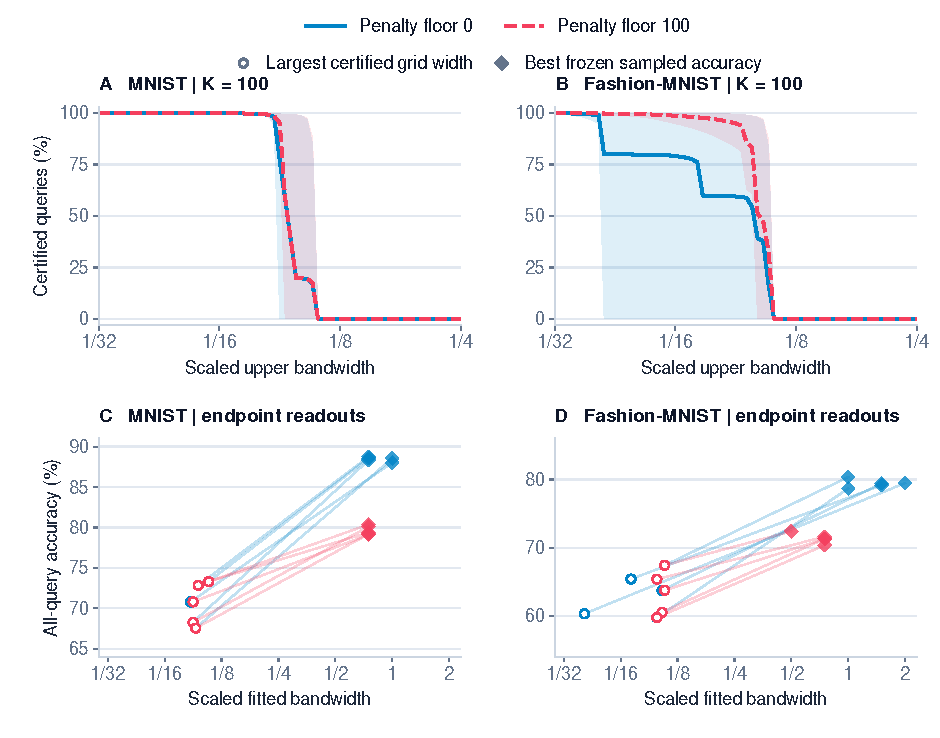
\includegraphics[width=\textwidth]{Figure_05_Certified_Frontier_Accuracy.pdf}
\caption{Post hoc certification frontiers and fitted accuracy at $K=100$. Columns correspond to the two datasets; colors identify penalty floors 0 and 100. Top panels show sharp coverage over the 67-width grid: lines are unweighted five-seed means and bands span seed minima and maxima. Bottom panels show individual seed observations at $\lambda=\lambda_0$. Open circles mark each seed's largest grid width retaining any certification; filled diamonds mark its highest-accuracy frozen sampled width. Thin segments pair observations from the same seed and floor. All accuracies use the complete evaluation set. The reference maximum is descriptive and is selected from 16 previously probed widths. Widths are divided by $s_C$; each observed certificate transition has an upper-to-lower bracket ratio no greater than 1.0321.}
\label{fig:frontier}
\end{figure}

At $K=100$ and floor zero, the mean largest passing grid width is $0.09323s_C$ on MNIST and $0.08370s_C$ on Fashion-MNIST. The corresponding mean readout accuracies are 70.55\% and 63.32\%, compared with sampled reference means of 88.45\% and 79.42\%. Table~\ref{tab:frontier} reports all floors, including paired accuracy differences. Raising the floor to 100 moves the Fashion-MNIST frontier range upward, while its mean frontier accuracy remains 63.37\%.

\begin{table}[!htbp]
\centering\small
\caption{Frontier and readout accuracy at $K=100$. The width range spans the five seeds' largest grid widths with any sharp certification. Accuracy columns are percentages, and the paired difference is in percentage points (pp); entries give five-seed means $\pm$ sample standard deviations. ``Reference'' is the highest observed accuracy among 16 frozen sampled widths at the same penalty.}
\label{tab:frontier}
\begin{tabular}{@{}lrcccc@{}}
\toprule
Dataset & $\lambda_0$ & Frontier $t/s_C$ & Accuracy (\%) & Reference (\%) & Difference (pp) \\
\midrule
MNIST & 0 & $0.0856$--$0.1068$ & $70.55\pm2.60$ & $88.45\pm0.27$ & $17.90\pm2.54$ \\
 & 1 & $0.0884$--$0.1068$ & $70.55\pm2.60$ & $87.97\pm0.31$ & $17.42\pm2.53$ \\
 & 100 & $0.0884$--$0.1068$ & $70.55\pm2.60$ & $79.64\pm0.57$ & $9.09\pm2.56$ \\
Fashion-MNIST & 0 & $0.0402$--$0.1068$ & $63.32\pm3.28$ & $79.42\pm0.62$ & $16.10\pm2.87$ \\
 & 1 & $0.0501$--$0.1068$ & $63.33\pm3.28$ & $78.23\pm0.61$ & $14.90\pm2.80$ \\
 & 100 & $0.0972$--$0.1068$ & $63.37\pm3.23$ & $71.39\pm0.73$ & $8.03\pm2.59$ \\
\bottomrule
\end{tabular}
\end{table}

The stored per-query brackets retain all censoring. Across the 15 groups per dataset, each floor has two left-censored sharp query/group records for MNIST; Fashion-MNIST has 124, 108, and 95 at floors 0, 1, and 100, respectively. No query is right-censored. These counts reuse evaluation images across seeds and prototype budgets. The original masks at $s_C/16$, $s_C/8$, and $s_C/4$ reproduce exactly, every numerical nesting check passes, and all certified supplementary endpoint predictions agree with their nearest-prototype labels.

The denser grid also resolves differences between the two class-wise bounds. Among 6,030 width--floor--group conditions, 35 have more sharp-certified queries than basic-certified queries. The total gain is 827 repeated query-condition records: 811 at floor one and 16 at floor 100. The largest single-condition gain is 382 Fashion-MNIST queries, or 3.82 percentage points. At floor zero the bounds coincide throughout. This supplementary finding retains the original grid's identical-mask result.
